\documentclass{article}
\usepackage[utf8]{inputenc}
\usepackage{graphicx}
\usepackage[italian]{babel}                   			% italian / english
\usepackage{amsmath}


\graphicspath{ {img/} }


\numberwithin{figure}{section}
\numberwithin{equation}{section}


\renewcommand{\figurename}{Figura}
\renewcommand{\familydefault}{\sfdefault}


\title{Fisica dei processi fotovoltaici}
\author{Com. Ale Smareglia}
\date{July 2016}

\begin{document}
\maketitle

\section{Introduzione}
Nel 1990 il consumo totale di energia era di 12 TW per 5.3 miliardi di persone. Per il 2050 le stime prevedono consumi di 28 TW per n totale di 8-10 miliardi di persone, sebbene siano stime il significato è chiaro: la domanda di energia è destinata ad aumentare. D'altro canto le fonti di energia non rinnovabili, come petrolio, gas, carbone e uranio sono limitate e destinate ad esaurirsi.\\
Il consumo di combustibili è descritto dalla curva di Hubbert, un geofisico che negli anni '60 lavorara per la Shell. La sua curva descrive la produzione di petrolio (ma vale per qualsiasi combustibile) nel tempo. La curva è definita come la derivata dell'equazione logistica: 
\begin{equation}
   Q(t)=\frac{Q_{\infty}}{1+e^{A(\tau_m-t)}} 
\end{equation}
dove $Q_\infty$ è il limite asintotico della curva. La curva logistica descrive una crescita autolimitata come nel caso in cui una popolazione abbia accesso a risorse limitate.

\begin{figure}[h!]
    \centering
    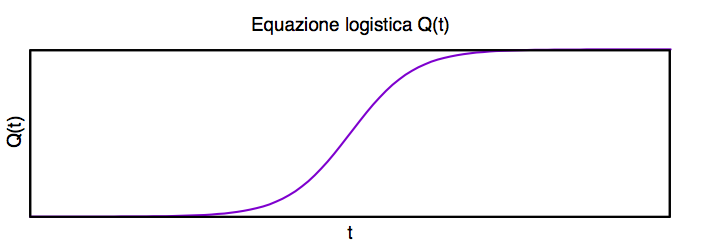
\includegraphics{logistica.png}
    \caption{Equazione logistica}
    \label{fig:logistica}
\end{figure}
La curva di Hubbert quindi è:
\begin{equation}
P_H = \frac{dQ}{dt} = AQ_\infty\frac{e^{A(\tau_m-t)}}{[1+e^{A(\tau_m-t)}]^2}
\end{equation}
che ha un andamento a campana molto simile ad una gaussiana. La parte "in salita" descrive quando vengono trovati nuovi giacimenti, man mano che l'estrazione diventa sempre più difficoltosa e costosa la curva rallenta e si appiattisce.

\begin{figure}[h!]
    \centering
    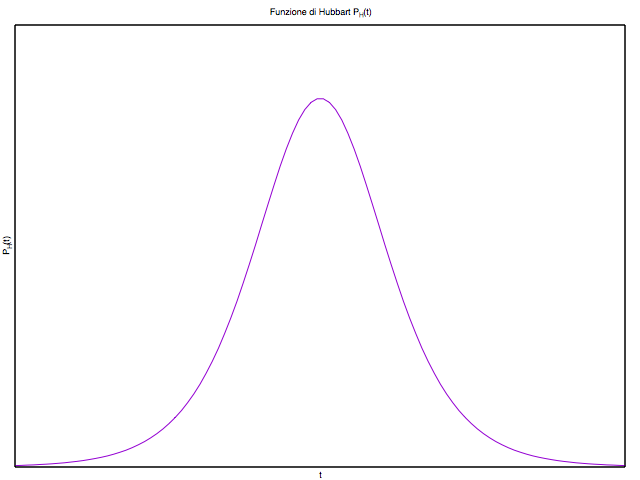
\includegraphics[scale=.4]{hub.png}
    \caption{Equazione di Hubbert}
    \label{fig:hub}
\end{figure}
Quando metà delle risorse sono state estratte si raggiunge il picco della curva, dopodiché c'è una fase di decrescita che ha lo stesso ritmo di quella di crescita, dando luogo così ad una curva simmetrica. Nel mondo reale non c'è alcun motivo per cui la curva debba essere simmetrica, anzi, spesso la decrescita è più lenta della fase di crescita a causa di interventi esterni come ad esempio politiche "di contenimento" volte a limitare il problema.
Al 2001 le previsioni di questo modello, integrate con dati reali, danno una stima del picco attorno al 2040. Questo fa abbastanza riflettere se si tiene conto che il nel 2011 il 90\% dell'energia è prodotto da combustibili fossili.\\

L'energia nucleare potrebbe essere una temporanea alternativa al petrolio, anche se implica profonde considerazioni socioeconomiche e geopolitiche come ad esempio la gestione delle scorie e l'eventuale uso dei reattori per produrre materiale fissile per scopi militari. In ogni caso le riserve di uranio sono limitate e quindi il nucleare non può essere considerato una fonte rinnovabile.\\

Il carbone è disponibile in grandi giacimenti ma non infiniti. Bruciare carbone produce molta energia ma al tempo stesso genera grandi quantità di biossido di carbonio e altri gas serra. I problemi derivanti dall'uso del carbone erano già noti nel 1273, anno in cui venne promulgata la prima legge anti inquinamento della storia: veniva fatto divieto di bruciare carbone nella città di Londra. Un'altra conseguenza dell'uso del carbone fu la diminuzione della popolazione di falene bianche dovuta all'annerimento delle betulle durante la rivoluzione industriale.\\

Esiste una roadmap sulle emissioni di carbonio che prevede di aumentare il PIL senza aumentare le emissioni di carbonio. Non tutti i paesi seguono questa linea di sviluppo, anzi quelli con più risorse tendono a farne un uso meno efficiente (ad esempio USA/Canada e paesi arabi).
Negli anni '70 una previsione sul raggiungimento del picco della curva di Hubbert attorno agli anni 2000 diede inizio alla crisi petrolifera. Nuovi giacimenti e nuove tecniche vennero sviluppati e il problema venne solo posticipato. Al giorno d'oggi è improbabile che si verifichino ancora nuove scoperte di grandi giacimenti.\\

Il sole produce un sacco di energia, circa 170 PW. In media sulla terra arrivano 1000 W/m\textsuperscript{2} di energia che in condizione nuvolose o di elevato inquinamento atmosferico (come nelle grandi città) possono scendere facilmente a 10 W/m\textsuperscript{2}. Una stima prevede che coprendo lo 0.16\% della superficie terrestre (circa una volta e mezzo l'area occupata dalla Francia) con pannelli solari con efficienza del 6\% si produrrebbero 20TW, cioè il fabbisogno energetico stimato per il 2050.
La radiazione solare è, al momento, l'unica fonte di energia pulita e rinnovabile che proviene da un reattore a fusione, il Sole. L'energia solare può essere convertita in calore (solare termodinamico), può essere usata per produrre idrogeno o trasformata in energia elettrica.\\

Il processo di conversione della luce in energia venne scoperto da Becquerel. Smith scoprì che il selenio se illuminato poteva produrre elettricità nel 1873. Tre anni dopo un suo studente realizzò una giunzione selenio-platino fotovoltaica. In ogni caso il fotovoltaico rimase una curiosità finchè non arrivarono i primi prototipi in silicio che garantivano efficienze di conversione del 6\%.





\end{document}
